\documentclass[11pt]{article}
\usepackage[margin=1in]{geometry}
\usepackage[latin2]{inputenc}
\usepackage[english]{babel}
\usepackage[cmex10]{amsmath}
\usepackage{amsthm}
\usepackage{amssymb}
\usepackage{xspace}
\usepackage{cite}
\usepackage{tikz}
\usepackage{comment}
\usepackage{caption}
\usepackage{subcaption}
\usepackage{letltxmacro}
\usepackage{comment}
\usetikzlibrary{snakes}

\newtheorem{theorem}{Theorem}[section]
\newtheorem{lemma}[theorem]{Lemma}
\newtheorem{claim}[theorem]{Claim}
\newtheorem{corollary}[theorem]{Corollary}
\newtheorem{proposition}[theorem]{Proposition}
\newtheorem{observation}[theorem]{Observation}
\theoremstyle{definition}
\newtheorem{definition}[theorem]{Definition}
\newtheorem{example}[theorem]{Example}

\newcommand{\cF}{{\mathcal{F}}}
\newcommand{\cg}{G_{\cF_0}}

\newcommand{\pw}{\ensuremath{\mathtt{pw}}\xspace}
\newcommand{\poly}{\mathrm{poly}}
\newcommand{\dist}{\mathrm{dist}}
\newcommand{\Oh}{\ensuremath{\mathcal{O}}}
\newcommand{\Ohstar}{\ensuremath{\Oh^\star}}

\def\cqedsymbol{\ifmmode\else{\unskip\nobreak\hfil
\penalty50\hskip1em\null\nobreak\hfil
\parfillskip=0pt\finalhyphendemerits=0\endgraf}\fi} 

\newcommand{\cqed}{\renewcommand{\qed}{\cqedsymbol}}


\newcommand{\executeiffilenewer}[3]{\ifnum\pdfstrcmp{\pdffilemoddate{#1}}{\pdffilemoddate{#2}}>0{\immediate\write18{#3}}\fi } 
\newcommand{\includesvg}[1]{\executeiffilenewer{figures/#1.svg}{figures/#1.pdf}{inkscape -z -D --file=figures/#1.svg --export-pdf=figures/#1.pdf --export-latex}{\input{figures/#1.pdf_tex}}}
\newcommand{\svg}[2]{\def\svgwidth{#1}\includesvg{#2}}

\renewcommand{\topfraction}{0.85}
\renewcommand{\textfraction}{0.1}
\renewcommand{\floatpagefraction}{0.75}

\newcommand{\tudu}[1]{{\bf{TODO: #1}}}

\newcommand{\defproblem}[3]{
  \vspace{1.5mm}
\noindent\fbox{
  \begin{minipage}{16cm}
  #1 \\
  {\bf{Input:}} #2  \\
  {\bf{Question:}} #3
  \end{minipage}
  }
  \vspace{1.5mm}
}

\newcommand{\defproblemG}[3]{
  \vspace{2mm}
\noindent\fbox{
  \begin{minipage}{16cm}
  #1 \\
  {\bf{Input:}} #2  \\
  {\bf{Goal:}} #3
  \end{minipage}
  }
  \vspace{2mm}
}

\newcommand{\pathdecomp}{\mathbb{P}\xspace}

\DeclareMathAlphabet{\mathcal}{OMS}{cmsy}{m}{n}
\renewcommand{\S}{{\mathcal S}}
\renewcommand{\H}{{\mathcal H}}

\newcommand{\probshort}{\textsc{PDDPP}}
\newcommand{\probname}{\textsc{Planar Directed Disjoint Paths Problem}}

\newcommand{\MC}{{\textsc{Multicolored Clique}}\xspace}
\newcommand{\kSP}{{\textsc{-Set Packing}}\xspace}
\newcommand{\SP}{{\textsc{Set Packing}}\xspace}
\newcommand{\tSP}{{\textsc{-Set Packing}}\xspace}
\newcommand{\tDM}{{\textsc{-Dimensional Matching}}\xspace}
\newcommand{\kDM}{{\textsc{-Dimensional Matching}}\xspace}

\newcommand{\group}{\Lambda}
\newcommand{\vnoose}{\vec{\nu}}
\newcommand{\snoose}{\vec{\mu}}
\newcommand{\alt}{\mathfrak{a}}
\newcommand{\Z}{\mathbb{Z}}
\newcommand{\R}{\mathbb{R}}
\newcommand{\disccomp}{\ensuremath{\anycomp^{\textrm{disc}}}}
\newcommand{\ringcomp}{\ensuremath{\anycomp^{\textrm{ring}}}}
\newcommand{\decomp}{\ensuremath{\mathcal{D}}}
\newcommand{\incarcs}[1]{\ensuremath{\hat{E}(#1)}}

\newwrite\tempfile
\immediate\openout\tempfile=references.txt
\newcommand{\writeref}[1]{\immediate\write\tempfile{\unexpanded{#1}}}
\newcommand{\writerefe}[1]{\immediate\write\tempfile{\expandafter{#1}}}
\LetLtxMacro{\oldref}{\ref}
\LetLtxMacro{\oldsection}{\section}
\renewcommand{\ref}[1]{\oldref{#1}\writeref{\oldref{#1} (#1)}\writeref{}}


\title{Improved approximation for -dimensional matching \\via bounded pathwidth local search\thanks{The preliminary version of this paper was presented at the 54th Annual IEEE Symposium on Foundations of Computer Science (FOCS'13). The author is partially supported by
Foundation for Polish Science grant HOMING PLUS/2012-6/2.}}

\author{Marek Cygan
  \thanks{
    Institute of Informatics, University of Warsaw, Poland,
      \texttt{cygan@mimuw.edu.pl}.
  }
}

\begin{document}

\maketitle

\begin{abstract}
One of the most natural optimization problems is the \kSP problem,
where given a family of sets of size at most  one
should select a maximum size subfamily of pairwise disjoint sets.
A special case of -{\sc Set Packing} is the 
well known \tDM problem, which is a maximum hypermatching problem in -uniform tripartite hypergraphs.
Both problems belong to the Karp's list of  NP-complete problems.
The best known polynomial time approximation ratio for \kSP
is  and goes back to 
the work of Hurkens and Schrijver~[SIDMA'89], which gives -approximation for \tDM.
Those results are obtained by a simple local search algorithm,
that uses constant size swaps.


The main result of this paper is a new approach to local search for \kSP
where only a special type of swaps is considered, 
which we call swaps of bounded pathwidth.
We show that for a fixed value of  one can search the space of -size
swaps of constant pathwidth in  time.
Moreover we present an analysis proving that
a local search maximum with respect to -size swaps of
constant pathwidth yields a polynomial time -approximation
algorithm, improving the best known approximation
ratio for \kSP. In particular we improve the approximation
ratio for \tDM from  to .
\end{abstract}

\section{Introduction}

In the \SP problem, also known as {\sc Hypergraph Matching}, we are given a family  
of subsets of , and the goal is to find a maximum size
subfamily of  of pairwise disjoint sets.
\SP is a fundamental problem in combinatorial optimization
with various applications.
A simple reduction from {\sc Independent Set} (where )
combined with the hardness result of H{\aa}stad~\cite{haastad}
makes the \SP problem hard to approximate.
When each set of \SP is of size at most 
the problem is denoted as \kSP.

\defproblemG{\kSP}{A family  of sets of size at most .}
{Find a maximum size subfamily of  of pairwise disjoint sets.}

\kSP is a generalization of {\sc Independent Set} in bounded degree graphs,
  as well as -{\sc Dimensional Matching} and is related to plethora of other problems
(see~\cite{lau} for a list of connections between
 \kSP and other combinatorial optimization problems).
In \tDM the universe  is partitioned into 
and  is a subset of .

Both \tDM and \SP are 
well studied problems, belonging to Karp's list of 21 NP-hard problems~\cite{karp21}.
A simple greedy algorithm returning any inclusionwise maximal
subfamily of disjoint subsets of  gives a -approximation
for \kSP.
One can consider a local search routine, where 
as long as it is possible we remove one set from our current feasible solution
and add two new sets.
We say that such an algorithm uses size  swaps, as two new sets are involved.
It is known that a local search maximum with respect to size  swaps
is a -approximation for \kSP.
If, instead of using swaps of size  we use swaps of 
size  for bigger values of , then the approximation
ratio approaches , and that is exactly
the -approximation algorithm by Hurkens and Schrijver~\cite{hs89}.

Despite significant interest (see Section~\ref{sec:related})
for over  years no improved polynomial time approximation
algorithm was obtained for \kSP, even for the special case of \tDM.
Meanwhile Halld{\'o}rsson~\cite{h95}\footnote{Similar arguments
 were also used by Berman and F{\"u}rer~\cite{berman-furer} for the
   independent set problem in bounded degree graphs.} has shown
that a local search maximum with respect to  size
swaps gives a -approximation, which was recently
improved to ~\cite{cgm13}.
Nevertheless enumerating all  size swaps 
takes quasipolynomial time.

\subsection{Our results and techniques}

Based on the work of Halld{\'o}rsson~\cite{h95}
a natural path to transforming a quasipolynomial
time approximation into a polynomial time approximation
would be by designing a~ time algorithm,
where  is a constant.
This is exactly the framework of parameterized complexity\footnote{For further information about parameterized
  complexity we defer the reader to monographs~\cite{fpt1,fpt2,fpt3}.},
where the swap size is a natural parameter.
Unfortunately, we show that this is most likely impossible, i.e. there is no
such algorithm with  running time, unless W[1]=FPT,
where  is some computable function, even for .
We would like to note that W[1]FPT is a widely believed assumption,
in particular if W[1]=FPT, then the Exponential Time Hypothesis of~\cite{eth} fails.

\begin{theorem}
\label{thm:w1-intro}
Unless , there is no  time algorithm, that given a family 
of sets of size  and its disjoint subfamily 
either finds a bigger disjoint family  or verifies
that there is no disjoint family  such that ,
\end{theorem}

Therefore trying to find a  time algorithm which searches the whole
-size swaps space is not the proper path.
For this reason we introduce a notion of swaps (also called improving sets)
of bounded pathwidth (see Section~\ref{ssec:improving}).
Intuitively a size  swap is of bounded pathwidth,
if the bipartite graph where vertices represent sets that are added and removed,
and edges correspond to  non-empty intersections, is of constant pathwidth.
Using the color-coding technique of Alon et al.~\cite{color-coding}
we show that one can search the space of swaps of size at most  of bounded pathwidth in  time, for a constant .
As the currently best known analysis of local search maximum with respect to logarithmic size swaps of~\cite{cgm13}
relies on swaps of unbounded pathwidth,
we need to develop a different proof strategy, and the core part of
it is contained in Lemma~\ref{lem:improving-tree}.
The algorithm and its analysis complete the main result of this paper,
that is a polynomial time -approximation algorithm,
for any fixed  and~.

\begin{theorem}
\label{thm:main}
For any  and any integer 
there is a polynomial time -approximation algorithm
for \kSP.
\end{theorem}

We believe that the usage of parameterized tools
such as color-coding, pathwidth and W[1]-hardness in the
setting of this work is interesting on its own,
as to the best of our knowledge such tools
have not been previously used in local search based approximation algorithms.

\subsection{Related work}
\label{sec:related}

Even though there was no improvement 
in terms of polynomial time approximation of \kSP (and \tDM)
since the work of Hurkens and Schrijver~\cite{hs89},
both problems are well studied.


One can also consider weighted variant of \kSP,
where we want to select a maximum weight disjoint subfamily of .
Arkin and Hassin~\cite{arkin-hassin}
gave a -approximation algorithm,
Chandra and Halld{\'o}rsson~\cite{chandra-halldorson}
improved it to -approximation,
later improved by Berman~\cite{berman} to -approximation.
All the mentioned results are based on local search.

Also for the standard (unweighted) \kSP problem
Chan and Lau~\cite{lau} presented a strengthened
LP relaxation, which has integrality gap .

On the other hand, Hazan et al~\cite{hazan}
have shown that \kSP is hard to approximate within a factor of . 
Concerning small values of , Berman and Karpinski~\cite{berman-karpinski}
obtained a  hardness for \tDM, while
Hazan et al.~\cite{hazan2} obtained , , and  hardness
for ,  and -{\sc Dimensional Matching} respectively (note that a hardness result for \kDM
directly gives a hardness for \kSP).

Recently Sviridenko and Ward~\cite{sviridenko-ward} have
independently obtained a -approximation algorithm for \kSP.
They observed that the analysis of Halld{\'o}rsson~\cite{h95} 
can be combined with a clever application of the color coding
technique. However to the best of our understanding 
it is not possible to obtain -approximation
for \kSP using the tools of~\cite{sviridenko-ward},
and in particular Sviridenko and Ward do not improve the
approximation ratio for .
The main difference between this article and~\cite{sviridenko-ward}
is in handling sets of the optimum solution, that
intersect exactly one set in a local maximum.

\subsection{Organisation}

We start with preliminaries in Section~\ref{sec:preliminaries},
where we recall standard graph notation together
with the definition of pathwidth and path decompositions.

Section~\ref{sec:main} contains the main result of this paper,
that is the -approximation for \kSP.
First, we introduce the notion of improving set of bounded
pathwidth in Section~\ref{ssec:improving}.
In Section~\ref{ssec:algorithm} we apply the color coding 
technique to obtain a polynomial time algorithm
searching an improving set of logarithmic size
of bounded pathwidth.
In Section~\ref{ssec:analysis} we analyse a local search
maximum with respect to bounded pathwidth improving sets of
logarithmic size.
The heart of our analysis is contained in 
an abstract combinatorial Lemma~\ref{lem:improving-tree}
which is later applied in the proof of Lemma~\ref{lem:analysis}.

The proof of Theorem~\ref{thm:w1-intro} is given
in Section~\ref{sec:hardness}.
Finally, in Section~\ref{sec:conclusions} we conclude
with potential future research directions.

\section{Preliminaries}
\label{sec:preliminaries}

We use standard graph notation. For an undirected graph  by  and 
we denote the set of its vertices and edges respectively. By 
we denote the open neighborhood of a vertex , while the closed neighborhood is defined as .
Similarly, for a subset of vertices  we have  and .

By a disjoint family of sets we denote a family, where each pair of sets is pairwise disjoint.
For a positive integer  by  we denote the set .

\paragraph{Pathwidth and path decompositions} A \emph{path decomposition} of a graph~ is a sequence~, where each
set  is a subset of vertices~ (called a \emph{bag}) such that~ and the following properties hold:
\begin{itemize}
\item[(i)] For each edge~ there is a bag  in~ such that~.
\item[(ii)] If~ then~ for each .
\end{itemize}

The \emph{width} of~ is the size of the largest bag minus one, and the {\em pathwidth} of a graph~ is the minimum width over all possible path decompositions of~. Since our focus here is on path decompositions we only mention in passing that the related notion of \emph{treewidth} can be defined similarly, except for letting the bags of the decomposition form a tree instead of a path.

In order to make the description easier to follow,
it is common to use path decompositions that adhere to some simplifying properties.
The most commonly used notion is that of a nice path decompositions, introduced by Kloks~\cite{Kloks94}; the main idea is that adjacent nodes can be assumed to have bags differing by at most one vertex. 

\begin{definition}[{\bf nice path decomposition}] \label{def:nicepathdecomp}
A \emph{nice path decomposition} is a path decomposition , where each bag is of one of the following types:
\begin{itemize}
\item \textbf{First (leftmost) bag}: the bag  is empty,~.
\item \textbf{Introduce bag}: an internal bag~ of  with predecessor~ such that~ for some . 
This bag is said to \emph{introduce} .
\item \textbf{Forget bag}: an internal bag~ of  with predecessor~ for which  for some . This bag is said to \emph{forget} .
\item \textbf{Last (rightmost) bag}: the bag associated with the largest index, i.e. , is empty,~.
\end{itemize}
\end{definition}

It is easy to verify that any given path decomposition can be transformed in polynomial time into a nice path decomposition without increasing its width.

\section{Local search algorithm}
\label{sec:main}

In this section we present the main result of the paper,
i.e. the -approximation algorithm for \kSP,
proving Theorem~\ref{thm:main}.
We start with introducing the notion of improving set of bounded
pathwidth in Section~\ref{ssec:improving}.
Next, in Section~\ref{ssec:algorithm} we apply the color coding 
technique to obtain a polynomial time algorithm
searching an improving set of logarithmic size
of bounded pathwidth.
In Section~\ref{ssec:analysis} we analyse a local search
maximum with respect to bounded pathwidth improving sets of
logarithmic size.
The heart of our analysis is contained in 
an abstract combinatorial Lemma~\ref{lem:improving-tree}
which is later applied in the proof of Lemma~\ref{lem:analysis}.

\subsection{Bounded pathwidth improving set}
\label{ssec:improving}

Let us assume that an instance  of \kSP is given.
Moreover by  we denote some disjoint subfamily of ,
which we can think of as a current feasible solution of a local search algorithm.
In what follows we define a {\em conflict graph}, which
is a bipartite undirected graph with two independent sets of vertices being  and ,
where an edge reflects non-empty intersection.

\begin{definition}[{\bf conflict graph}]
For a disjoint family  by a {\em conflict graph}  we denote
an undirected bipartite graph with vertex set  and edge set .
\end{definition}

Next, we define an {\em improving set} , which
can be used to increase the cardinality of , and then we introduce 
a notion of an {\em improving set of bounded pathwidth}, which will be crucial in 
both the algorithm and the analysis of its approximation ratio.

\begin{definition}[{\bf improving set}]
\label{def:improving}
For a disjoint family  a set 
is called an {\em improving set}, if the following conditions hold:
\begin{itemize}
  \item all sets of  are pairwise disjoint,
  \item , i.e. the number of sets of  having a common
  element with at least one set of  is strictly smaller than .
\end{itemize}
\end{definition}

Observe, that if we have an improving set , then 
is a disjoint subfamily of  of size greater than , hence the name improving set.

\begin{definition}[{\bf improving set of bounded pathwidth}]
An improving set  with respect to  has {\em pathwidth at most },
if the subgraph of the conflict graph  induced by  has pathwidth at most .
\end{definition}

\subsection{Algorithm}
\label{ssec:algorithm}

To find an improving set of bounded pathwidth we use
the color coding technique of Alon et al.~\cite{color-coding},
which is by now a well-established tool in parameterized complexity
used for finding a set consisting of disjoint objects.
We use two random colorings , ,
where  ensures that the sets of  are disjoint,
while  is used not to consider the same set of  twice.

\begin{lemma}
\label{lem:search}
There is an algorithm, that given a disjoint family ,
and two coloring functions , 
in  time determines, whether there exists an improving 
set  of size at most 
of pathwidth at most , such that  is injective on  
and  is injective on .
\end{lemma}

\begin{proof}
For the sake of notation by adding dummy distinct elements we ensure 
that each set of  has size exactly~.
Define an auxiliary directed graph ,
where each vertex is characterized by a subset of set colors ,
a subset of element colors , and a subset of  of size at most ,
i.e.  

Note that this graph has  vertices.

Since there will be no possibility of confusion, to make the proof easier
to follow by  for  we denote ,
i.e. we omit the subscript .
The idea behind the construction is that each vertex of  describes
a potential prefix of a sequence of bags in a path decomposition of 
for some .
The set  encodes the set of vertices of  in the current bag
and ensures the bounded pathwidth property.
Instead of storing all the sets of  that have already appeared in the 
sequence of bags, we store only the colors of the elements of  (encoded by~),
as it is enough to maintain the disjointness of sets of 
and keep track of the cardinality of  - due to the assumption that each 
set of is size exactly~.
Similarly instead of storing all the sets of 
that were already introduced, we only store their colors (encoded by~).

To the set  we add the following arcs.
For , 
such that :
\begin{itemize}
  \item if , ,  is injective on  
  and ,
  then add to  an arc 
  \item if ,  and for each  
  either , or ,
  then add to  an arc 
\end{itemize}

To the set  we add the following arcs.
For ,   add to 
an arc  
if one of the following conditions holds:
\begin{itemize}
  \item ,
  \item  and .
\end{itemize}

\begin{claim}
There exists a path in the graph  from the vertex 
to a vertex  for 
iff
there exists an improving set  of size at most  of pathwidth at most ,
such that  is injective on  and  is injective on .
\end{claim}

\begin{proof}
Assume that there is a path  in ,
where ,  ,  and .
Let .
By construction of , we have .
By the definition of  and 
since , at the time a vertex  appears
for the first time in some  we ensure that all its neighbors in 
are either in  or are colored by  with colors not yet in .
Moreover at the time  is forgotten, i.e. removed from some ,
we ensure that all of its neighbors in  have been already added to bags.
Therefore  and for each 
edge  of  the endpoints of  appear in some bag .
Since no set of  is added twice, due to the coloring ,
no set of  is added twice, due to the coloring ,
 is a path decomposition of  of width at most .
Finally .
Hence  is an improving set of size at most  and of pathwidth at most .

In the other direction, let  be an improving set of size at most  
such that  is injective on ,  is injective on ,
and let  be a nice path decomposition of  of width at most .
For  define  as ,
where .
Observe that ,  for 
and moreover if  is an introduce bag, then 
while if  is a forget bag, then .
Consequently there is a path from  to  in the graph .

\end{proof}

By the above claim it is enough to run a standard graph
search algorithm, to check whether there exists a path
from the vertex 
to  where ,
which finishes the proof of Lemma~\ref{lem:search}.
\end{proof}

\begin{theorem}
\label{thm:search}
There is an algorithm, that given a disjoint family ,
in  time determines, whether there exists an improving 
set  of size at most 
of pathwidth at most .
\end{theorem}

\begin{proof}
Observe, that if we take 
where the color of each set is chosen uniformly and independently at random,
then for an improving set  of size at most  
the function  is injective on 
with probability at least 
Similarly, if we assign a color of  to each element of ,
then with probability at least  the function  is injective on .
Therefore invoking Lemma~\ref{lem:search} with random colorings  at least  
times would yield a constant error probability.

To obtain a deterministic algorithm we can use the, by now standard, technique of splitters.  An -splitter is a family  of functions , such that for any  of size at most  there exists  that is injective on .  What we need is a small family of -splitters.

\begin{theorem}[ \hskip -0.25cm \cite{opt-splitters}]
\label{thm:splitters}
There exists an -splitter of size 
that can be constructed in  time.
\end{theorem}

Therefore instead of using random colorings ,  we can use Theorem~\ref{thm:splitters}
to construct  and  splitters, leading to a deterministic algorithm,
which finishes the proof of Theorem~\ref{thm:search}.
\end{proof}

\subsection{Analysis}
\label{ssec:analysis}

In this subsection we analyze a local search maximum, with respect
to logarithmic size improving sets of constant pathwidth.
It is well known that an undirected graph of average degree
at least  contains a cycle of length at most ,
   where the constant  depends on .
This observation was the base for the quasipolynomial time algorithms of~\cite{h95,cgm13}.
Here, however we need to generalize this result extensively,
as the analysis of~\cite{cgm13} relies on improving sets of unbounded pathwidth.

Throughout this subsection we operate on multigraphs, as there might be several
parallel edges in a graph, however there will be no self-loops.

\begin{lemma}
\label{lem:improving-tree}
Let  be an -vertex undirected multigraph of minimum degree at least .
Assume that each edge  is associated with a subset of an alphabet  of size at most , where .
If each element  appears in at most  sets , i.e. , then
there exists a tree , which is a subgraph of , and a vertex , such that:
\begin{itemize}
  \item ;
  \item there exist two edges  which have both endpoints in ;
  \item  is a tree with at most  leaves; 
  \item for each pair of edges  such that 
  we have , where ,
  and .
\end{itemize}
\end{lemma}

\begin{proof}
First we deal with some corner cases. 
\begin{itemize}
\item[(i)] If in  there are three parallel edges  between vertices  and ,
then as  we take  and set , .
\item[(ii)] If in  there are three vertices , two parallel edges  between  and 
as well as two parallel edges  between  and , 
than as  we take  and set , .
\item[(iii)] In the last corner case let us assume that for each vertex  of 
there are some two parallel edges  incident to .
Let  be any edge of  for which there is no parallel edge in  -
such an edge exists, as otherwise  or  would hold.
Let  be a vertex such that in  there are two parallel edges  between  and ,
similarly let  be a vertex such that in  there are two parallel edges  between  and .
Observe that  as otherwise case (ii) would hold.
In that case ,  and .
\end{itemize}
Assuming that none of , ,  holds,
there is a vertex  in , which is adjacent to at least three distinct vertices .

We are going to construct a sequence of logarithmic number of trees  rooted at , which are subgraphs of  satisfying two invariants:
\begin{itemize}
  \item {\bf (exponential growth)} for any  the number of vertices in 
  at distance exactly  from  is exactly ,
  and there are no vertices at distance more than ,
  \item{\bf (-nearness)} for any two edges  of  if ,
  then .
\end{itemize}
We will show, that having constructed a tree  for some  we
can either construct a tree  satisfying the two invariants,
or find a tree  with edges  required by the claim of the lemma.

Let  and note that it satisfies the two invariants.
Assume, that  (for some ) was the most recently constructed tree,
and we want to construct .
Let  be the vertices of  at distance exactly  from the root .
By the exponential growth invariant we have .
Let  be the set of edges of  incident to , but not contained in .
As each vertex in  is of degree at least three, we have

Let 
i.e. the set of edges having a non-empty intersection with , where  is not contained
in the last  levels of .  Observe that for  the set  is empty.
When extending the tree  to maintain the -nearness invariant,
we use only edges of .

Let .
We consider two cases: either 
or not. In the former case we will show that one can construct a tree  satisfying both exponential growth and -nearness invariants.
In the latter case we will show that the required tree  and edges  exist.

If ,
then we select exactly  vertices out of 
and extend the tree  to  by adding one more layer of vertices (at distance  from ),
connected to vertices of  by edges of .
Clearly the exponential growth invariant is satisfied for . 
Furthermore, since  satisfied the -nearness invariant
and by the definition of  the tree  also satisfies the -nearness invariant.

In the remaining part of the proof we assume 

and show the required tree  with edges .
If at least two edges of  have both endpoints in ,
denote those edges , then as  we take the subtree of  induced
by vertices on the paths between  and their least common ancestor 
and set ,  (see Figure~\ref{fig3}).
Therefore let  be the subset of edges having
exactly one endpoint in  (that is in ).
By~(\ref{eq0}) we infer that


\begin{figure}
\begin{center}
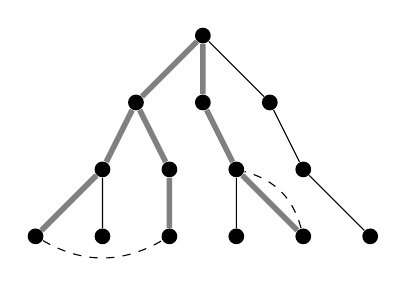
\begin{tikzpicture}[scale=0.85]
  \tikzstyle{vertex}=[circle,fill=black,minimum size=0.20cm,inner sep=0pt]
  \tikzstyle{vertex2}=[circle,draw=black,fill=gray!50,minimum size=0.20cm,inner sep=0pt]
 	\tikzstyle{vertex3}=[circle,draw=black,fill=white,minimum size=0.20cm,inner sep=0pt]
 
  \tikzstyle{terminal}=[rectangle,draw=black,fill=white,minimum size=0.2cm,inner sep=0pt]

\node[vertex] (v0) at (0,0){};
\node[vertex] (v1) at (-1,-1){};
\node[vertex] (v2) at (0,-1){};
\node[vertex] (v3) at (1,-1){};


\node[vertex] (v4) at (-1.5,-2){};
\node[vertex] (v5) at (-0.5,-2){};
\node[vertex] (v6) at (0.5,-2){};
\node[vertex] (v7) at (1.5,-2){};

\node[vertex] (v8) at (-2.5,-3){};
\node[vertex] (v9) at (-1.5,-3){};
\node[vertex] (v10) at (-0.5,-3){};
\node[vertex] (v11) at (0.5,-3){};
\node[vertex] (v12) at (1.5,-3){};
\node[vertex] (v13) at (2.5,-3){};

\draw (v1) -- (v0) -- (v2);
\draw (v0) -- (v3);

\draw (v4) -- (v1) -- (v5);
\draw (v6) -- (v2);
\draw (v7) -- (v3);

\draw(v8) -- (v4) -- (v9);
\draw (v10) -- (v5);
\draw (v11) -- (v6) -- (v12);
\draw (v13) -- (v7);

\draw[dashed] (v8) edge[bend right] (v10);
\draw[dashed] (v12) edge[bend right] (v6);

\draw[color=gray,line width=2] (v8) -- (v4) -- (v1) -- (v0);
\draw[color=gray,line width=2] (v10) -- (v5) -- (v1);

\draw[color=gray,line width=2] (v12) -- (v6) -- (v2) -- (v0);

\end{tikzpicture}
 \end{center}
\caption{Edges of the tree  are gray, while edges  and  are dashed.}
\label{fig3}
\end{figure}

Let  be a maximum size subset of , such
that no two edges of  have a common endpoint in .
Observe that if , then either:
\begin{itemize}
  \item there exists three edges  having a common endpoint in , or
  \item there exist four edges , such that  have a common endpoint in 
  and  have a common endpoint in .
\end{itemize}
In both cases we can extend the tree  by one or two edges to construct
 and set ,  (see Figure~\ref{fig4}).

\begin{figure}
\begin{center}
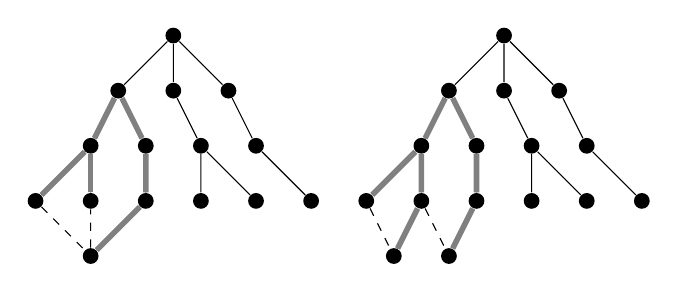
\begin{tikzpicture}[scale=0.70]
  \tikzstyle{vertex}=[circle,fill=black,minimum size=0.20cm,inner sep=0pt]
  \tikzstyle{vertex2}=[circle,draw=black,fill=gray!50,minimum size=0.20cm,inner sep=0pt]
 	\tikzstyle{vertex3}=[circle,draw=black,fill=white,minimum size=0.20cm,inner sep=0pt]
 
  \tikzstyle{terminal}=[rectangle,draw=black,fill=white,minimum size=0.2cm,inner sep=0pt]


\node[vertex] (v0) at (0,0){};
\node[vertex] (v1) at (-1,-1){};
\node[vertex] (v2) at (0,-1){};
\node[vertex] (v3) at (1,-1){};


\node[vertex] (v4) at (-1.5,-2){};
\node[vertex] (v5) at (-0.5,-2){};
\node[vertex] (v6) at (0.5,-2){};
\node[vertex] (v7) at (1.5,-2){};

\node[vertex] (v8) at (-2.5,-3){};
\node[vertex] (v9) at (-1.5,-3){};
\node[vertex] (v10) at (-0.5,-3){};
\node[vertex] (v11) at (0.5,-3){};
\node[vertex] (v12) at (1.5,-3){};
\node[vertex] (v13) at (2.5,-3){};

\draw (v1) -- (v0) -- (v2);
\draw (v0) -- (v3);

\draw (v4) -- (v1) -- (v5);
\draw (v6) -- (v2);
\draw (v7) -- (v3);

\draw(v8) -- (v4) -- (v9);
\draw (v10) -- (v5);
\draw (v11) -- (v6) -- (v12);
\draw (v13) -- (v7);

\node[vertex] (x) at (-1.5,-4){};
\draw[dashed] (v8) -- (x) -- (v9);
\draw (x) -- (v10);

\draw[color=gray,line width=2] (v8) -- (v4) -- (v1);
\draw[color=gray,line width=2] (v9) -- (v4);
\draw[color=gray,line width=2] (x) -- (v10) -- (v5) -- (v1);


\begin{scope}[xshift=6cm]
\node[vertex] (v0) at (0,0){};
\node[vertex] (v1) at (-1,-1){};
\node[vertex] (v2) at (0,-1){};
\node[vertex] (v3) at (1,-1){};


\node[vertex] (v4) at (-1.5,-2){};
\node[vertex] (v5) at (-0.5,-2){};
\node[vertex] (v6) at (0.5,-2){};
\node[vertex] (v7) at (1.5,-2){};

\node[vertex] (v8) at (-2.5,-3){};
\node[vertex] (v9) at (-1.5,-3){};
\node[vertex] (v10) at (-0.5,-3){};
\node[vertex] (v11) at (0.5,-3){};
\node[vertex] (v12) at (1.5,-3){};
\node[vertex] (v13) at (2.5,-3){};

\draw (v1) -- (v0) -- (v2);
\draw (v0) -- (v3);

\draw (v4) -- (v1) -- (v5);
\draw (v6) -- (v2);
\draw (v7) -- (v3);

\draw(v8) -- (v4) -- (v9);
\draw (v10) -- (v5);
\draw (v11) -- (v6) -- (v12);
\draw (v13) -- (v7);

\node[vertex] (x) at (-2,-4){};
\node[vertex] (y) at (-1,-4){};
\draw[dashed] (v8) -- (x) -- (v9) -- (y);


\draw[color=gray,line width=2] (v8) -- (v4) -- (v1);
\draw[color=gray,line width=2] (x) -- (v9) -- (v4);
\draw[color=gray,line width=2] (y) -- (v10) -- (v5) -- (v1);
\end{scope}

\end{tikzpicture}
 \end{center}
\caption{Creating the tree  assuming . Notation as in Figure~\ref{fig3}.}
\label{fig4}
\end{figure}

Consequently we have , which together with~(\ref{eq2}) gives


In the last part of the proof we use the following claim.
\begin{claim}
\label{claim:bound}

\end{claim}
\begin{proof}
Recall that if , the set  is empty.
Hence by inequality~(\ref{eq3}) in that case .
A direct check shows that for each  we have ,
which proves the claim in the case .

When  we have 


Finally for  we upper bound the size of 

The first inequality follows from the assumption, that each set  is of size at most  and each element of 
is contained in at most  sets , hence each of  contributes at most  edges to .
The last inequality follows from the choice of  and the assumption .
Therefore 

\end{proof}

Observe that by the definition of  we have ,
but then Claim~\ref{claim:bound} contradicts inequality~(\ref{eq1}).
\end{proof}

\begin{corollary}
\label{cor:decomposition}
Let  be an undirected multigraph with  vertices
and of minimum degree at least .
Assume that each edge  is associated with a subset of an alphabet  
of size at most , for some , such that each element of  appears in at most  sets .
There exists a subgraph  of , and a path decomposition  of 
 of width at most , where  and 
\begin{itemize}
  \item[(a)] ,
  \item[(b)] ,
  \item[(c)]  for each pair of edges , such that 
  there exists a bag  for some , such that all of the endpoints of both  and  are contained
  in ,
  \item[(d)] for each edge  the set of indices 
  is an interval.
\end{itemize}
\end{corollary}

\begin{proof}
First, we use Lemma~\ref{lem:improving-tree} to obtain , , such that 
, where for each pair of edges  such that 
we have .
Let  be two edges with both endpoints in .
Define , clearly  is a subgraph of 
and the number of edges is the number of vertices plus one.
Therefore properties  and  are satisfied and
it remains to show that there exists a path decomposition of  of width at most ,
satisfying  and .

Let  be the set of vertices of  at distance exactly  from 
 in .
Consider a sequence , where ,
and .
It is straightforward to check that this is in fact a path decomposition of ,
and since  has at most  leaves, this implies that the size of each 
is upper bounded by , and hence the path decomposition is of width
at most~.

Observe that property  required by the corollary follows from
the last property of Lemma~\ref{lem:improving-tree},
because all of the endpoints of edges , such that ,
are contained in .
To prove property  let  be an arbitrary edge of 
and define  and .
As we already know that  is a path decomposition
it follows that both sets ,  form an interval,
hence  is also an interval, which proves .
\end{proof}

\begin{lemma}
\label{lem:analysis}
Fix an arbitrary . 
There are constants  (depending on  and ),
such that for any disjoint family ,
for which there is no improving set of size at most  of pathwidth at most 
we have ,
where  is a maximum size disjoint subfamily of .
\end{lemma}

\begin{proof}
Let  and denote , .
Let  be the subgraph of  induced by .
We are going to construct a sequence of at most  subgraphs of ,
namely  for , where , , 
satisfying two invariants:
\begin{itemize}
 \item[(a)] in  there is no subset  of size at most , such that ,
 \item[(b)] .
\end{itemize}
Observe  trivially satisfies 
and in order to make  satisfy  
it is enough to set  and  so that

as there is no improving set of size at most 
and pathwidth of an improving set of size  is at most .
Consider subsequent values of  starting from .
Split the vertices of  into groups , 
consisting of vertices of  of degree exactly one, exactly two and at least three in , respectively.
Observe that because of  there is no isolated vertex of  in 
and moreover no two vertices of  have a common neighbour in .
Consider the following two cases:
\begin{itemize}
  \item :
  in this case we construct a graph , where
   and . 
  The invariant  is satisfied, as any set  of size at most  
  such that  would imply existence of 
  a set  of size at most ,
  such that  (see Figure~\ref{fig1}).
  \begin{figure}
  \begin{center}
  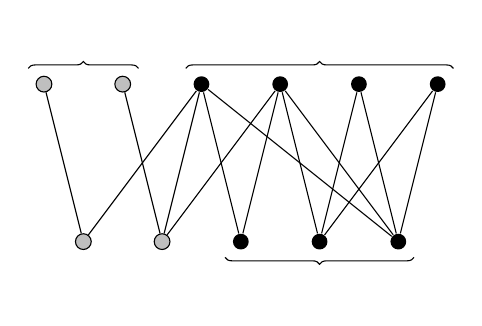
\begin{tikzpicture}[scale=1]
  \tikzstyle{vertex}=[circle,fill=black,minimum size=0.20cm,inner sep=0pt]
  \tikzstyle{vertex2}=[circle,draw=black,fill=gray!50,minimum size=0.20cm,inner sep=0pt]
  \tikzstyle{terminal}=[rectangle,draw=black,fill=white,minimum size=0.2cm,inner sep=0pt]


	\foreach \x in {2,3,4,5}
	{
		\node[vertex] (a\x) at (\x,2){};
	}
	\node[vertex2] (a0) at (0,2){};
	\node[vertex2] (a1) at (1,2){};

	\foreach \x in {2,3,4}
	{
		\node[vertex] (b\x) at (\x+0.5,0){};
	}
	\node[vertex2] (b0) at (0.5,0){};
	\node[vertex2] (b1) at (1.5,0){};
		

	\draw (a1) -- (b1);
	\draw (a0) -- (b0);
	\draw (a2) -- (b2);
	\draw (a2) -- (b4);
	\draw (a2) -- (b0);
	\draw (a2) -- (b1);
	\draw (a3) -- (b1);
	\draw (a3) -- (b4);
	\draw (a3) -- (b3);

\draw (a3) -- (b2);
\draw (a4) -- (b4);
\draw (a4) -- (b3);
\draw (a5) -- (b4);
\draw (a5) -- (b3);

\draw[snake=brace] (1.8,2.2) -- (5.2,2.2);
\draw (3.5,2.6) node {};

\draw[snake=brace] (-0.2,2.2) -- (1.2,2.2);
\draw (0.5,2.6) node {};

\draw[snake=brace] (4.7,-0.2) -- (2.3,-0.2);
\draw (3.5,-0.6) node {};


\end{tikzpicture}
   \end{center}
  \caption{Lifting an improving set  in  to an improving set  in . Gray vertices belong to  but not to .}
  \label{fig1}
  \end{figure}
  \item :
  We are going to use the following claim, which we prove later.
  \begin{claim}
  \label{claim:new}
  
  \end{claim}

  As each vertex of  is of degree at most  in ,
  the number of edges of  is at most .
  At the same time the number of edges of  is at least 
  , therefore
  

  Note that summing the inequalities:
  
   we obtain

   
   However , 
   where the second equality follows from invariant ,
   hence .
\end{itemize}
In the second case we have proved the thesis, while the first case can 
appear only  number of times, as in each step we remove at least  vertices from .
Therefore to finish the proof of Lemma~\ref{lem:analysis} it suffices to prove Claim~\ref{claim:new}.
\end{proof}

\begin{proof}[Proof of Claim~\ref{claim:new}]
Assume the contrary.
Construct a multigraph , where .
Set  and for each edge ,  set as  the set of
all vertices of  at distance at most  from .
Observe that since  is of maximum degree at most , we have .
For the same reason each vertex of  appears in at most  sets .

In order to use Corollary~\ref{cor:decomposition} we need to reduce the graph ,
in a way ensuring all its vertices are of degree at least .
However we know, that the graph  is of average degree at least , since .
Let . As long as there exist an isolated vertex, or a vertex of degree one in  remove it.
Note that such a reduction rule does not decrease the average degree of .
Similarly if  contains a path ,
where all vertices  for  are of degree exactly  and ,
then remove all the vertices  for  from .
As this operation removes  vertices, but only  edges, and ,
the average degree does not decrease.
Finally, we construct  from  by simultaneously considering
all the maximal paths , with all internal vertices of degree two,
and contracting each of such paths to a single edge  and setting . 
Observe that for each edge  of  the size of  is upper bounded by ,
as a contracted path consist of at most  edges.

As  is of minimum degree at least , we apply Corollary~\ref{cor:decomposition} 
to it, where .
Let  and  be
as defined in Corollary~\ref{cor:decomposition}.
Let  be the set of all the vertices of  corresponding to the edges of ,
including the vertices of  that correspond to edges of  that were contracted into
some edge of  (see Figure~\ref{fig2}).
As  we have .
Clearly  is of size at most ,
that is logarithmic in , as  is a constant.
It remains to show that we can lift  to an improving set
of bounded pathwidth, while increasing its size only by a constant factor.

\begin{figure}
\begin{center}
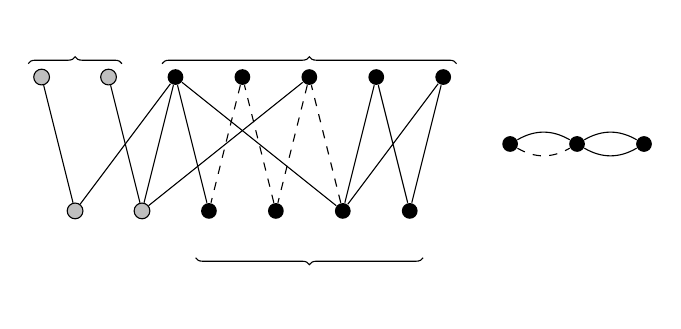
\begin{tikzpicture}[scale=0.85]
  \tikzstyle{vertex}=[circle,fill=black,minimum size=0.20cm,inner sep=0pt]
  \tikzstyle{vertex2}=[circle,draw=black,fill=gray!50,minimum size=0.20cm,inner sep=0pt]
 	\tikzstyle{vertex3}=[circle,draw=black,fill=white,minimum size=0.20cm,inner sep=0pt]
 
  \tikzstyle{terminal}=[rectangle,draw=black,fill=white,minimum size=0.2cm,inner sep=0pt]


\node[vertex2] (a0) at (0,2){};
\node[vertex2] (a1) at (1,2){};
\node[vertex] (a2) at (2,2){};
\node[vertex] (a3) at (3,2){};
\node[vertex] (a4) at (4,2){};
\node[vertex] (a5) at (5,2){};
\node[vertex] (a6) at (6,2){};

\node[vertex2] (b0) at (0.5,0){};
\node[vertex2] (b1) at (1.5,0){};
\node[vertex] (b2) at (2.5,0){};
\node[vertex] (b3) at (3.5,0){};
\node[vertex] (b4) at (4.5,0){};
\node[vertex] (b5) at (5.5,0){};

\draw (a5) -- (b4) -- (a6) -- (b5) -- (a5);
\draw[dashed] (b4) -- (a4) -- (b3) -- (a3) -- (b2);
\draw (b2)-- (a2) -- (b4);

\draw (a0) -- (b0);
\draw (a1) -- (b1);
\draw (b0) -- (a2) -- (b1) -- (a4);	

\draw[snake=brace] (1.8,2.2) -- (6.2,2.2);
\draw (4,2.6) node {};

\draw[snake=brace] (-0.2,2.2) -- (1.2,2.2);
\draw (0.5,2.6) node {};

\draw[snake=brace] (5.7,-0.7) -- (2.3,-0.7);
\draw (4,-1.2) node {};

\draw (2.5,-0.4) node {};
\draw (4.5,-0.4) node {};
\draw (5.5,-0.4) node {};


\node[vertex] (a) at (7,1){};
\node[vertex] (b) at (8,1){};
\node[vertex] (c) at (9,1){};
\draw (a) edge[bend left] (b);
\draw[dashed] (a) edge[bend right] (b);
\draw (b) edge[bend left] (c);
\draw (b) edge[bend right] (c);
\draw (7,0.6) node {};
\draw (8,0.6) node {};
\draw (9,0.6) node {};
\draw (8,1.5) node {};

\end{tikzpicture}
 \end{center}
\caption{The right graph is  provided by Corollary~\ref{cor:decomposition}.
  The left side depicts the set  corresponding to , as well as lifting the set  to . Gray vertices belong to  but not to . The dashed path on the left between  and  in  is contracted into an edge of  on the right.}
\label{fig2}
\end{figure}

Let . For  set  (see Figure~\ref{fig2}).
Observe that at each step the size of  increases by a factor of at most ,
hence  and moreover  is an improving set w.r.t. .
Since  is of size logarithmic in  it remains to show that 
is of constant pathwidth.

Create a sequence of subsets , by taking as 
the set .
The size of each  is at most , where 
is the width of , hence it remains to show that 
is indeed a path decomposition.
Each vertex of  is within distance at most 
from some vertex of , hence each vertex of  
is contained in some set  for .
Similarly each edge of  is within distance
at most  from some vertex of , so it has both its endpoints
in some set  for .
Since  is a path decomposition each edge 
has both its endpoints in some bag~, therefore

and each edge of  has both its endpoints in some bag .
 Property (d) of Corollary \ref{cor:decomposition} implies
 that each  contributes to  for values of  forming
 an interval . Moreover if for two edges 
 the intersection  is non-empty, then
 by property (c) of Corollary~\ref{cor:decomposition} we know
 that the intervals  and  have non-empty intersection.
 This ensures that each vertex  of  appears in a set of bags 
 forming an interval in the sequence ,
 as each pair of intervals in  has non-empty intersection.

Therefore  is an improving set of logarithmic size and 
of constant pathwidth, which is a contradiction. Consequently
, which finishes 
the proof of Claim~\ref{claim:new}.
\end{proof}

Lemma~\ref{lem:analysis} together with the algorithm
for searching improving sets of bounded pathwidth from Theorem~\ref{thm:search}
gives a polynomial time -approximation algorithm
for \kSP for any constant , proving Theorem~\ref{thm:main}.
In particular there is a -approximation for 
the \tDM problem.

\section{Local search hardness}
\label{sec:hardness}

In this section we are going to show, that there is no 
algorithm verifying for a given , whether there exists 
an improving set (see Definition~\ref{def:improving}) of size at most 
in  time, even when .
In fact we show a stronger hardness result, 
ruling out existence of an algorithm, that either 
finds a bigger disjoint family  (without any restriction
on its distance from ), or verifies that there is no
improving set of size at most .
That is exactly the notion of {\em permissive} parameterized local search
introduced by Marx and Schlotter in~\cite{permissive-ls} 
(for more information about parameterized local search see~\cite{fellows-ls,gaspers-ls,ls-survey}).

In our reduction, we use a standard W[1]-hard problem~\cite{mc-hardness}, namely \MC 
parameterized by the clique size.

\defproblem{\MC}{An undirected graph , a positive integer , and a color function .}
{Does the graph  contain a clique of size , where each vertex is of different color?}

\begin{theorem}
\label{thm:w1-hardness}
There is a constant , such that
given an instance  of \MC one can in polynomial time construct
an instance  of \tSP, together with a disjoint subfamily  of size , such that:
\begin{itemize}
  \item If  is a YES-instance, then there exists a family 
  of disjoint  sets, such that ,
  \item if there exists a disjoint subfamily  of size ,
  then  is a YES-instance.
\end{itemize}
\end{theorem}

\begin{proof}
We start with a definition of a simple gadget, that will be used a couple of times
in the construction.
\begin{definition}
For a positive integer  and a symbol  an -amplifier is a family  of sets of size~, where 

\end{definition}

Let  be an instance of \MC.
W.l.o.g. we may assume that , where  is a positive integer,
since otherwise we may add universal vertices (adjacent to all other vertices).
We start with constructing an -amplifier, which will
be called the {\em top amplifier},
and -amplifier for each , called {\em vertex amplifiers}.
As the universe  we take

To the family  we add all the sets of  and  for , as well as:
\begin{itemize}
  \item[(i)] sets  for ,
  \item[(ii)] sets  for  for ,
  \item[(iii)] sets  for , ,
  \item[(iv)] sets  for ,
  \item[(v)] sets  for  (note that ),
  \item[(vi)] consider all the elements  in lexicographic order of pairs ,
  take subsequent triples of elements and add them to the family , that is
  add sets 
  
  (note that , since ).
\end{itemize}

To finish the construction we create a disjoint family  of size  as follows:
\begin{itemize}
  \item add to  sets  for  such that  is odd.
  \item add to  sets  for  and , such that  is odd.
  \item add to  all the sets from points (i), (v), (vi) of the construction of .
\end{itemize}

Note that the size of  equals , as the only elements which are not covered by  are ,  and .

\begin{claim}
\label{claim:1}
If  is a YES-instance, then there exists a disjoint family  of size ,
such that .
\end{claim}

\begin{proof}
Let  be a solution to , that is a multicolored clique of size .
Construct a disjoint family  as follows:
\begin{itemize}
\item[(a)] add to  sets  for each , such that  is even,
\item[(b)] add to  sets  for  and , such that  is even,
\item[(c)] add to  sets  for  and , such that  is odd,
\item[(d)] for  add to  the set , where  is the unique vertex of  of color ,
\item[(e)] add to  sets  for ,
\item[(f)] add to  sets  for , ,
\item[(g)] add to  sets  for .
\end{itemize}
A direct check shows that the above family is disjoint and covers all the elements of , hence .
Note that in the above construction of  in each of the points (a), (d), (g) we add to  only  sets,
while in points (b), (f) we add to   sets, whereas
in points (c) and (e) we add to  sets that are present in . 
Therefore the number of sets of  which are not present in  is upper bounded by a linear function in .
\end{proof}

\begin{claim}
\label{claim:2}
If there exists a disjoint family  of size , then
 is a YES-instance.
\end{claim}

\begin{proof}
Let  be any disjoint family of size .
Since the element  can be covered only by the set , the family  contains
all the sets  for , where  is even,
and consequently elements  for  are not covered by sets of .
Therefore elements  are covered by sets
from point (ii) of the construction of ,
hence for each  in  there is exactly one set  for ,
and let  be the set of those  multicolored vertices.

We want to show that  is a clique.
As for each  we have , 
the family  contains all the sets 
for  where  is even.
Consequently elements  for , 
are covered by sets from point (iii) of the construction of .
Consider any pair .
Denote as  the unique vertex of 
and let  be the set of  covering , where .
This implies that  is not covered by a set of the -amplifier,
hence  is covered by the -amplifier, i.e. by .
Therefore  and the vertices of colors  and  of 
are adjacent.
Since  and  were selected arbitrarily,  is a clique.
\end{proof}

The proof of Theorem~\ref{thm:w1-hardness} follows from Claim~\ref{claim:1} and Claim~\ref{claim:2}.
\end{proof}

Theorem~\ref{thm:w1-hardness}, together with the well-known fact that \MC
is W[1]-hard~\cite{mc-hardness} implies Theorem~\ref{thm:w1-intro}.


\section{Future work and open problems}
\label{sec:conclusions}

One can try to continue the research direction
of Chan and Lau~\cite{lau}, who presented a
strengthening of the standard LP relaxation,
proving integrality gap of 
using a local search inspired analysis.
We would like to ask a question whether it is possible
to obtain some strengthened LP relaxation with integrality gap
-for some constant~.

Finally, we believe that it is worth looking into 
other problems, where local search algorithms were
applied successfully, such as {\sc -Median}~\cite{k-median}
or {\sc Restricted Max-Min Fair Allocation}~\cite{svensson}.
A potential goal would be to design improved approximation local search algorithms
using non-constant size swaps in the spirit of the framework of this paper.

\section*{Acknowledgements}

We would like to thank Marcin Mucha for helpful discussions.

\bibliographystyle{abbrv}
\bibliography{3dm}


\end{document}
